% ==========================================
% SEÇÃO 3: MODELOS ORIENTADOS AO USUÁRIO E TRANSMISSÃO
% ==========================================
\section[Modelos]{Modelos de Cor e Transmissão}

\begin{frame}{Modelos Orientados ao Usuário: HSV e HSL}
    \begin{columns}[T]
        \begin{column}{0.55\textwidth}
            \begin{itemize}
                \item \textbf{A Falha Cognitiva do RGB:} O cérebro humano não calcula cores somando intensidades de luz.
                \vspace{0.2cm}
                \item \textbf{Abstração de Uso Prático:}
                \begin{itemize}
                    \item Hue (Matiz).
                    \item Saturation.
                    \item Value / Lightness.
                \end{itemize}
                \vspace{0.2cm}
                \item \textbf{Aplicação em UI/UX:} Base para seletores de cor (\textit{Color Pickers}). O usuário escolhe a tonalidade e depois ajusta a variação de brilho e pureza.
            \end{itemize}
        \end{column}
        
        \begin{column}{0.45\textwidth}
            \begin{figure}
                \centering
                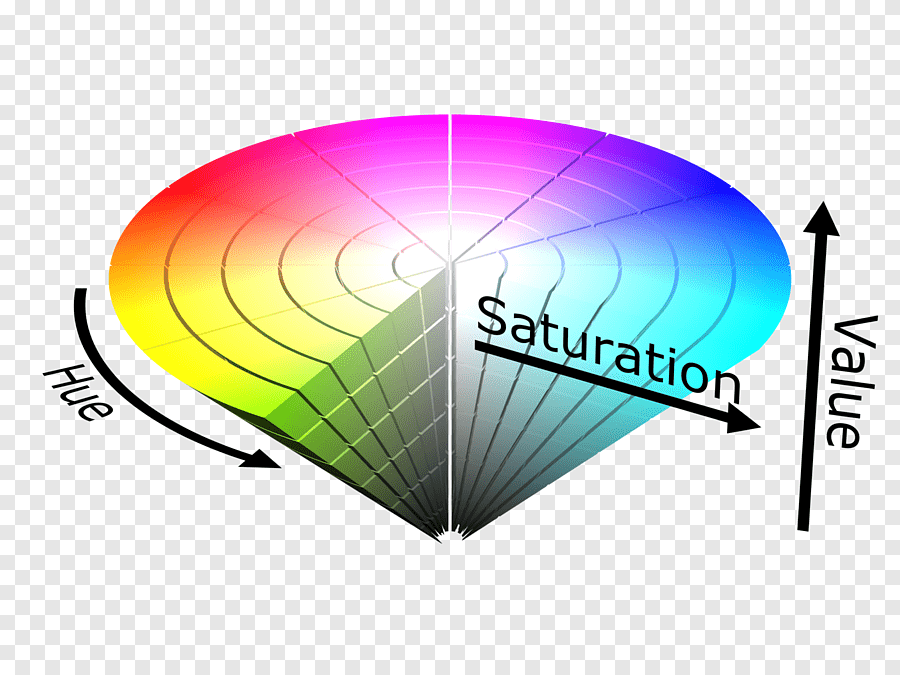
\includegraphics[width=0.9\textwidth]{images/cone_hsv.png}
                \caption{Espaço geométrico tridimensional do modelo HSV.}
            \end{figure}
        \end{column}
    \end{columns}

    \note{
        \begin{columns}[T]
            \begin{column}{0.49\textwidth}
                \scriptsize
                \textbf{RGB vs. HSV:} O RGB é um modelo de hardware, construído para otimizar o envio de sinal elétrico para subpixels na tela. O HSV e o HSL são modelos de software, construídos para alinhar a computação com a cognição visual humana.

                \textbf{Abstração de Uso Prático:}
                \begin{itemize}
                    \setlength{\itemsep}{1pt}
                    \item \textbf{Hue (Matiz):} A cor em si, mapeada em um círculo angular de 0° a 360° (onde 0° é Vermelho, 120° Verde, 240° Azul).
                    \item \textbf{Saturation:} O nível de pureza (0\% cinza absoluto, 100\% cor viva).
                    \item \textbf{Value / Lightness:} A quantidade de luz ou sombra injetada na cor.
                \end{itemize}
            \end{column}

            \begin{column}{0.51\textwidth}    
                \scriptsize
                \textbf{Engenharia de Software (UI):}
                \begin{itemize}
                    \setlength{\itemsep}{1pt}
                    \item \textbf{Aplicação em UI/UX:} Base para seletores de cor (\textit{Color Pickers}). O usuário escolhe a tonalidade e depois ajusta a variação de brilho e pureza.
                    \item \textbf{Conversão em Back-end:} Quando o usuário define a cor HSV interface, o programa converte para RGB antes de despachar para o barramento.
                \end{itemize}
                O cérebro humano não calcula cores somando intensidades de luz (ex: descobrir a mistura exata de R, G e B para gerar um tom de marrom).

                No HSV, $V=100\%$ é a cor pura (usado no Photoshop e Figma); no HSL, a cor pura fica em $L=50\%$, pois $L=100\%$ vira branco absoluto (padrão nativo na Web/CSS). O HSL é ideal na programação para criar paletas e \textit{Dark Mode} alterando apenas a variável $L$ aritmeticamente, sem quebrar o vetor de cor.
            \end{column}
        \end{columns}   
    }
\end{frame}

\begin{frame}{Transmissão e Processamento Cognitivo: YIQ e Cores Oponentes}
    \begin{columns}[T]
        \begin{column}{0.55\textwidth}
            \begin{itemize}
                \item \textbf{O Modelo YIQ e Engenharia de Software:}
                \begin{itemize}
                    \item \textbf{Criado para retrocompatibilidade.}
                    \item \textbf{Compressão de Banda:} O olho humano foca em detalhes no brilho ($Y$), não na cor.
                \end{itemize}

                \item \textbf{A Engenharia Biológica (Cores Oponentes):}
                \begin{itemize}
                    \item A retina converte os sinais de R, G e B em três eixos diferenciais de voltagem.
                \end{itemize}
            \end{itemize}
        \end{column}
        
        \begin{column}{0.45\textwidth}
            \begin{figure}
                \centering
                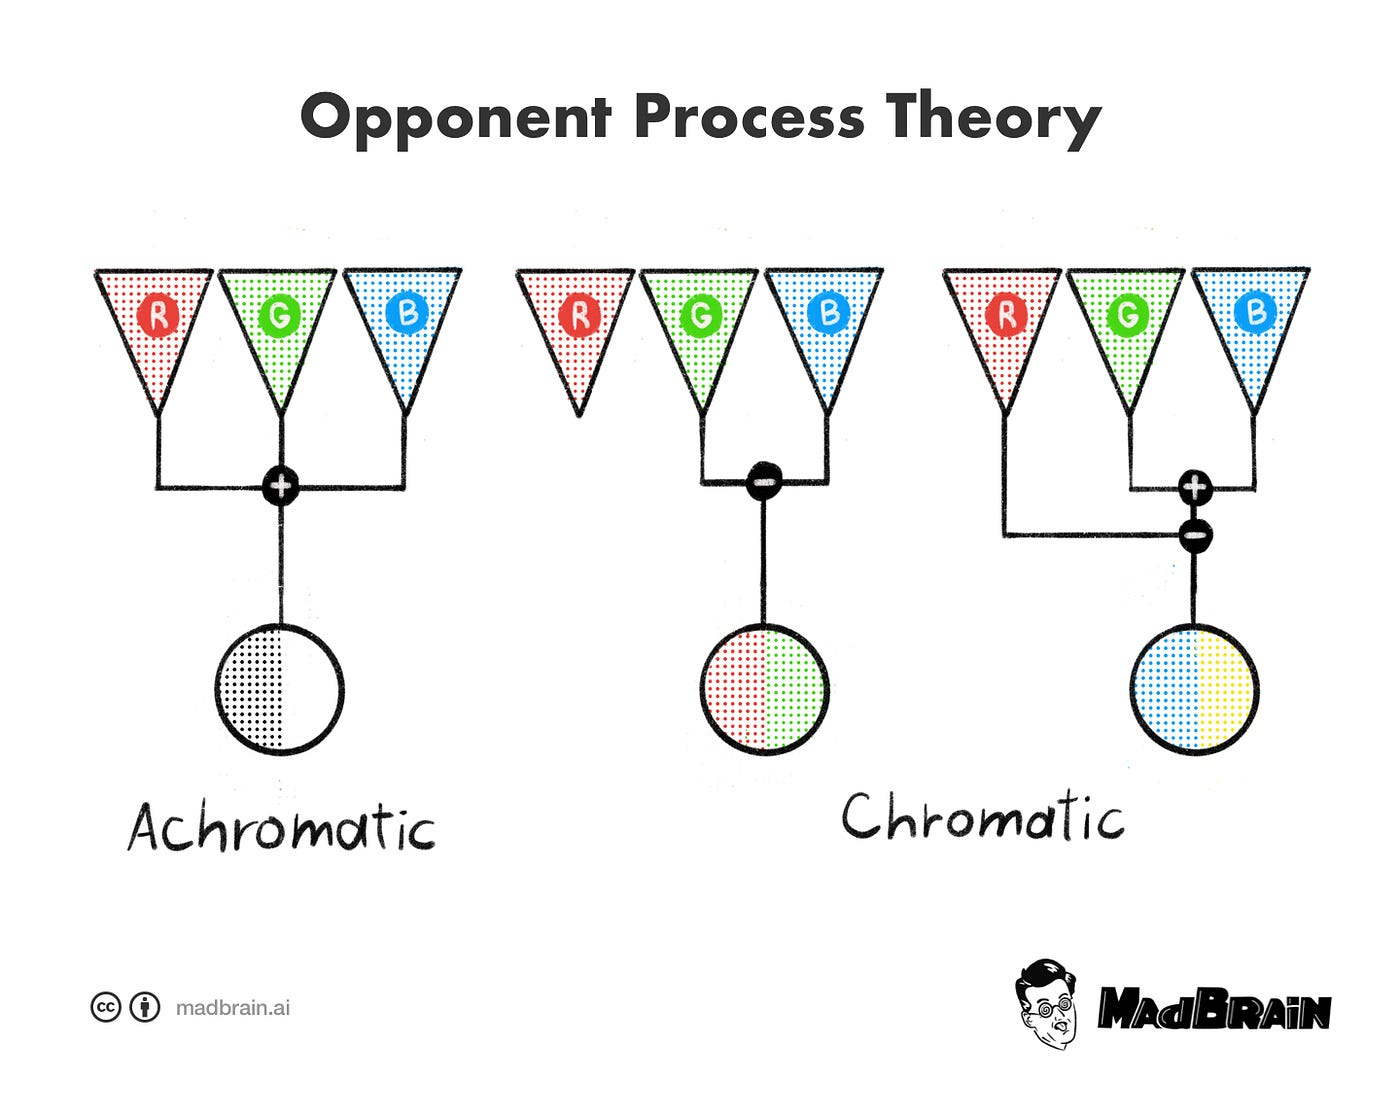
\includegraphics[width=0.9\textwidth]{images/teoria_oponentes.jpg}
                \caption{Esquema dos canais neurais oponentes e compressão de sinal.}
            \end{figure}
        \end{column}
    \end{columns}

    \note{
        \begin{columns}[T]
            \begin{column}{0.49\textwidth}
                \scriptsize
                \textbf{Otimização de Hardware e Banda:}
                \begin{itemize}
                    \setlength{\itemsep}{1pt}
                    \item \textbf{Subamostragem de Crominância:} O modelo YIQ é o ancestral direto dos formatos modernos de compressão de vídeo como YCbCr (usado em JPEG e MP4). O software descarta dados de cor porque a nossa acuidade visual para detalhes finos está concentrada quase que inteiramente na escala de cinza ($Y$).
                    \item O YIQ foi criado para retrocompatibilidade: TVs P\&B liam apenas o canal Y (Luminância/Brilho). TVs coloridas decodificavam I e Q (Crominância/Cor).
                    O olho humano foca em detalhes no brilho ($Y$), não na cor. Isso permitiu que engenheiros de transmissão reduzissem a largura de banda de $I$ e $Q$ pela metade sem perda de qualidade percebida.
                \end{itemize}
            \end{column}

            \begin{column}{0.51\textwidth}    
                \scriptsize
                \textbf{Mecânica Neurofisiológica:}
                \begin{itemize}
                    \setlength{\itemsep}{1pt}
                    \item \textbf{Fadiga de Receptores (Afterimage):} Olhar fixamente para uma imagem verde forte satura as células do oponente Verde. Ao olhar para uma parede branca, após isso, o receptor fadigado falha em disparar o sinal verde, fazendo com que o eixo oposto (Vermelho) dispare livremente. Gerando a ilusão de ver a mesma imagem em vermelho.
                \end{itemize}

                \textbf{A Engenharia Biológica (Cores Oponentes):}
                \begin{itemize}
                    \item A retina converte os sinais de R, G e B em três eixos diferenciais de voltagem: Vermelho-Verde, Azul-Amarelo e Claro-Escuro.
                    \item Como um sinal elétrico inibe o outro no mesmo canal, o cérebro não consegue processar "verde-avermelhado".
                \end{itemize}
            \end{column}
        \end{columns}   
    }
\end{frame}